\iffalse
\let\negmedspace\undefined
\let\negthickspace\undefined
\documentclass[journal,12pt,twocolumn]{IEEEtran}
\usepackage{cite}
\usepackage{amsmath,amssymb,amsfonts,amsthm}
\usepackage{algorithmic}
\usepackage{graphicx}
\usepackage{textcomp}
\usepackage{xcolor}
\usepackage{txfonts}
\usepackage{listings}
\usepackage{enumitem}
\usepackage{mathtools}
\usepackage{gensymb}
\usepackage{comment}
\usepackage[breaklinks=true]{hyperref}
\usepackage{tkz-euclide} 
\usepackage{listings}
\usepackage{gvv}                                        
\def\inputGnumericTable{}                                 
\usepackage[latin1]{inputenc}                                
\usepackage{color}                                            
\usepackage{array}                                            
\usepackage{longtable}                                       
\usepackage{calc}                                             
\usepackage{multirow}                                         
\usepackage{hhline}                                           
\usepackage{ifthen}                                           
\usepackage{lscape}
\usepackage{pgfplots}
\newtheorem{theorem}{Theorem}[section]
\newtheorem{problem}{Problem}
\newtheorem{proposition}{Proposition}[section]
\newtheorem{lemma}{Lemma}[section]
\newtheorem{corollary}[theorem]{Corollary}
\newtheorem{example}{Example}[section]
\newtheorem{definition}[problem]{Definition}
\newcommand{\BEQA}{\begin{eqnarray}}
\newcommand{\EEQA}{\end{eqnarray}}
\newcommand{\define}{\stackrel{\triangle}{=}}
\theoremstyle{remark}
\newtheorem{rem}{Remark}
\begin{document}

\bibliographystyle{IEEEtran}
\vspace{3cm}

\title{GATE 2022 IN 36}
\author{EE23BTECH11065 - prem sagar}
\maketitle
\newpage

\bigskip

\renewcommand{\thefigure}{\theenumi}
\renewcommand{\thetable}{\theenumi}
\textbf{Question}:
\\A signal $V_{in}\brak{t}$ shown is applied from t=0ms to t=6ms to the circuit shown Given the intial voltage across capacitor is 0.3V, and that the diode is ideal,the open circuit voltage $V_{out}\brak{t}$ at t=5ms is
\begin{figure}[h]
    \centering
    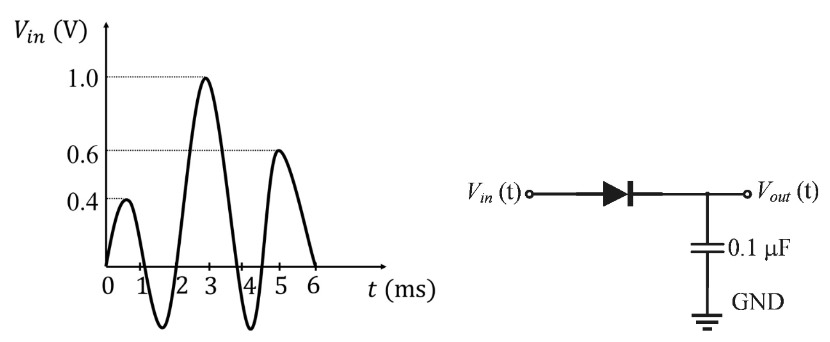
\includegraphics[width=1\linewidth]{2022/IN/36/figs/figuree.png}
    \caption{ }
\end{figure}
\begin{enumerate}
\item $0.3$v\\
\item $0.6$v\\
\item $0.7$v\\
\item $1.0$v\\
\end{enumarate}
\hfill{GATE 2022 IN}
\Solution
\fi
\begin{table}[!ht]
\def\arraystretch{1.5}
   \centering
      \begin{tabular}{|c|c|c|}
    \hline
            \textbf{Symbol} & \textbf{Value} & \textbf{Description} \\
    \hline
          $V_{in}\brak{t}$ &  & input signal\\
    \hline
          $V_c\brak{t}$ &  & voltage across capacitor\\
    \hline 
          $V_c\brak{0}$ &$0.3$V &intial voltage across capacitor\\
    \hline
          $v_{out}\brak{t}$ & &open circuit voltage\\
    \hline  
    $V_D$    & &Voltage across diode\\
    \hline
    $I_D$& &Diode current \\
    \hline
    $I_S$& &Saturation current \\
    \hline
    $V_T$&$\frac{kt}{q}$ &Thermal voltage \\
    \hline
  \end{tabular}

    \caption{input parameters}
 \end{table}
\\ the circuit is a positive peak detector circuit  
\begin{align}
I_D&=I_S\brak{e^\frac{V_D}{V_T}-1}
\end{align}
At t=3ms; $V_D>0$
\\$\therefore$ diode is forward biased
\begin{align}
\\V_{out}\brak{t}&=V_c\brak{t}
\\&=1V
\end{align}
After $t>3$ms; $V_D<0$
\\$\therefore$ diode is reverse biased
\\the capacitor voltage remains at 1V  
\\$\therefore$ at t=5ms
\begin{align}
V_{out}\brak{t}&=1V
\end{align}
\\\begin{figure}[h]
    \centering
    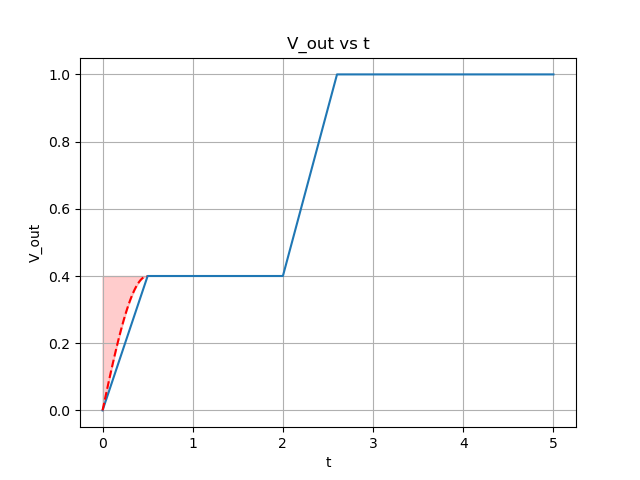
\includegraphics[width=1\linewidth]{2022/IN/36/figs/typo.png}
    \caption{ }
\end{figure}
%\end{document}
